\documentclass[sigconf,nonacm,screen]{acmart}
\usepackage{filecontents}
\usepackage{textcomp}
\usepackage{pgfplots}
\usetikzlibrary{patterns}
\usepackage{ifthen}
\usepgfplotslibrary{groupplots}
\RequirePackage{keyval}
\usepackage{multirow}
\usepackage{multicol}
\usepackage{csvsimple}
\usepackage[utf8]{inputenc}
\newcounter{row}
\newcounter{col}
\usepackage{wrapfig}
\usepackage{textgreek}
\usepackage[inline]{enumitem}
\usetikzlibrary{matrix, positioning}
\usetikzlibrary{patterns,tikzmark}
\usetikzlibrary{matrix,decorations.pathreplacing,calc}
\usepackage{hf-tikz}
\usepackage{pifont}
\usepackage{subfig}
\usetikzlibrary{chains,fit,shapes}
\usetikzlibrary{arrows.meta,
    chains,
    positioning,
    shapes.symbols}
\usetikzlibrary{decorations,calligraphy}
\usepackage{pgfplotstable}
\usepgfplotslibrary{statistics}
%\pgfplotsset{compat=newest}
\usetikzlibrary{matrix,calc}
\usetikzlibrary{fit}
\usepackage{xfp}
\usepackage{mathtools}

\usetikzlibrary{positioning}

\usepackage{makecell}
%\usepackage{tabu}
\usepackage{tikz}
\usetikzlibrary{trees}

%\pgfplotsset{compat=1.8}
\pgfplotsset{compat=1.12}


\usepgfplotslibrary{fillbetween}

\usepackage{filecontents}
% \usetikzlibrary{pgfplots.groupplots}
% \pgfplotsset{compat=1.9}

% \usepackage[utf8]{inputenc}
% \usepackage[ngerman]{babel}
% \usepackage{pgfplots}
% \pgfplotsset{compat=1.9}
% \usetikzlibrary{
%   pgfplots.groupplots,
%   matrix
% }
% \usepackage{siunitx}

\newtheorem{theorem}{Theorem}
\newtheorem{definition}{Definition}
\newcommand{\eat}[1]{}

\definecolor{bluegreen}{RGB}{3, 166, 155}
\definecolor{pitchblack}{RGB}{0, 0, 0}
\definecolor{lightbeige}{RGB}{255, 251, 241}
\definecolor{mediumgray}{RGB}{183, 183, 183}
\definecolor{mygreen}{rgb}{0,0.6,0}
\definecolor{mygray}{rgb}{0.5,0.5,0.5}
\definecolor{mymauve}{rgb}{0.58,0,0.82}
\definecolor{keywords}{RGB}{255,0,90}
\definecolor{comments}{RGB}{0,0,113}
\definecolor{red}{RGB}{255,0,0}
\definecolor{green}{RGB}{0,255,0}
\definecolor{navy}{RGB}{0,0,128}
\definecolor{DarkGrenen}{RGB}{0,100,0}
\definecolor{DarkOliveGreen}{RGB}{85,107,47}
\definecolor{saddlebrown}{RGB}{139,69,19}
\definecolor{gold}{RGB}{252,194,1}
\definecolor{tug}{RGB}{247,1,70}
\definecolor{tugb}{RGB}{120,137,251}


\definecolor{blue0}{RGB}{153,153,153}
\definecolor{blue1}{RGB}{77,77,77}%
\definecolor{blue2}{RGB}{165,71,209}
\definecolor{blue3}{RGB}{77,10,142}
\definecolor{blue4}{RGB}{74,139,203}
\definecolor{blue5}{RGB}{40,40,190}

\definecolor{color1}{RGB}{100,149,237} % corn flower blue
\definecolor{color2}{RGB}{153,153,153} % light gray
\definecolor{color3}{RGB}{0,0,0} % black
\definecolor{color4}{RGB}{255,165,0} % orange
\definecolor{color5}{RGB}{255,69,0} % orange red
\definecolor{color6}{RGB}{77,77,77} % dark gray
\definecolor{color7}{RGB}{31,119,180}
\definecolor{color8}{RGB}{7,77,125}
\definecolor{color9}{RGB}{153,216,201}


\definecolor{teal1}{RGB}{31, 111, 111}
\definecolor{teal2}{RGB}{84, 161, 161}
\definecolor{teal3}{RGB}{159, 200, 200}

\definecolor{dred1}{RGB}{160, 0, 0}
\definecolor{dred2}{RGB}{196, 102, 102}
\definecolor{dred3}{RGB}{216, 166, 166}


\definecolor{dblue1}{RGB}{32, 102, 168}
\definecolor{dblue2}{RGB}{53, 148, 204}
\definecolor{dblue3}{RGB}{140, 197, 227}

\definecolor{totalcolor}{RGB}{2, 152, 215}
\definecolor{mvcolor}{RGB}{248, 163, 47}
\definecolor{dvcolor}{RGB}{203, 70, 39}



% Enable this two commands when you want to extract diagrams in extra files, then run "make"
\usetikzlibrary{external}
\tikzexternalize[prefix=plots/] %  activate

\usetikzlibrary{positioning}

\sloppy
\clubpenalty = 10000
\widowpenalty = 10000
\brokenpenalty = 10000
\frenchspacing


\makeatletter
\def\pgfplots@drawaxis@lines@preparediscont@for#1{%
        \ifnum\csname pgfplots@#1axisdiscontnum\endcsname>0
                \begingroup
                % this group employs several temporary dimension registers
                % and is therefor scoped:
                \let\disstart=\pgf@ya
                \let\disend=\pgf@yb
                \disend=\csname pgfplots@#1max@reg\endcsname
                \advance\disend by -\csname pgfplots@#1min@reg\endcsname
                \disend=\csname pgfplots@#1@veclength\endcsname\disend
                \ifcase\csname pgfplots@#1axisdiscontnum\endcsname\relax
                        % has already been checked above.
                \or
                        \def\discontstyle{decoration={zigzag,segment length=5pt, amplitude=2pt}}%
                        \advance \disend by -8pt
                \or
                        \def\discontstyle{decoration={ticks,segment length=4pt, amplitude=8pt}}%
                        \advance \disend by -4pt
                \fi
                \pgfplotscoordmath{#1}{datascaletrafo get params}%
                % if #1max + shift < 0pt  (shift is 0 without the scaling trafo)
                \ifdim\csname pgfplots@#1max@reg\endcsname<-\pgfplotsretvalb pt
                        % swap start and end
                        \disstart=\disend
                        \disend=2pt
                \else
                        \disstart=2pt
                \fi
                % carry local computations outside of group:
                \xdef\pgfplots@glob@TMPa{%
                        \noexpand\def\expandafter\noexpand\csname #1disstart\endcsname{\the\disstart}%
                        \noexpand\def\expandafter\noexpand\csname #1disend\endcsname{\the\disend}%
                        \noexpand\pgfkeysdef{/tikz/#1discont}{\noexpand\pgfkeysalso{\discontstyle}}%
                }%
                \endgroup
                \pgfplots@glob@TMPa
        \else
                \expandafter\def\csname #1disstart\endcsname{0pt}%
                \expandafter\def\csname #1disend\endcsname{0pt}%
                \pgfkeyslet{/tikz/#1discont}=\pgfutil@empty
        \fi
}%
\makeatother



\begin{document}
\title[Query Processing by Data Catalog]{Query Processing by Data Catalog}

\author{Saeed Fathollahzadeh} 
\orcid{0000-0003-3723-6191}
\affiliation{
\institution{Concordia University}
\country{Canada}}

\renewcommand{\shortauthors}{Saeed Fathollahzadeh}

\maketitle

    % \tikzsetnextfilename{CatDB-Incremental-Binary_Abalone}
    % \begin{figure}[h]
    %     \centering
    %     \newcommand{\addplotCatDB}[7]{
	   \addplot[xshift=#1,draw=black,line width=0.15pt, fill=tug, discard if singlecatdb={#2}{#3}{#4},postaction={#5}] 
	   table[ y=Accuracy, col sep=comma, x=prompt_representation_type] {results/Experiment_CatDB_Micro_Benchmark.dat};
	   \label{leg_pip_accuracy}     
     
     \addplot[xshift=0pt,draw=black,line width=0.15pt, fill=tugb, fill opacity=1, discard if singlecatdb={#2}{#3}{#4},postaction={#5}] 
	   table[ y=F1_score, col sep=comma, x=prompt_representation_type] {results/Experiment_CatDB_Micro_Benchmark.dat};
	   \label{leg_pip_f1_score}     
};

\pgfplotsset{
    discard if singlecatdb/.style n args={3}{
        x filter/.code={
            \edef\tempa{\thisrow{llm_model}}
            \edef\tempb{#1}
            \ifx\tempa\tempb
                    \edef\tempc{\thisrow{task_type}}
                    \edef\tempd{#2}
                    \ifx\tempc\tempd
                      \edef\tempe{\thisrow{dataset}}
                      \edef\tempf{#3}
                      \ifx\tempe\tempf                        	
                      \else
                      \def\pgfmathresult{inf}
                      \fi
                    \else
                    \def\pgfmathresult{inf}
                    \fi      
            \else
            \def\pgfmathresult{inf}
            \fi			
        }
    },
    discard if singleautoml/.style n args={2}{
      x filter/.code={
          \edef\tempa{\thisrow{framework}}
          \edef\tempb{#1}
          \ifx\tempa\tempb
                  \edef\tempc{\thisrow{type}}
                  \edef\tempd{#2}
                  \ifx\tempc\tempd   
                  \else                
                  \def\pgfmathresult{inf}
                  \fi      
          \else
          \def\pgfmathresult{inf}
          \fi			
      }
  }
};

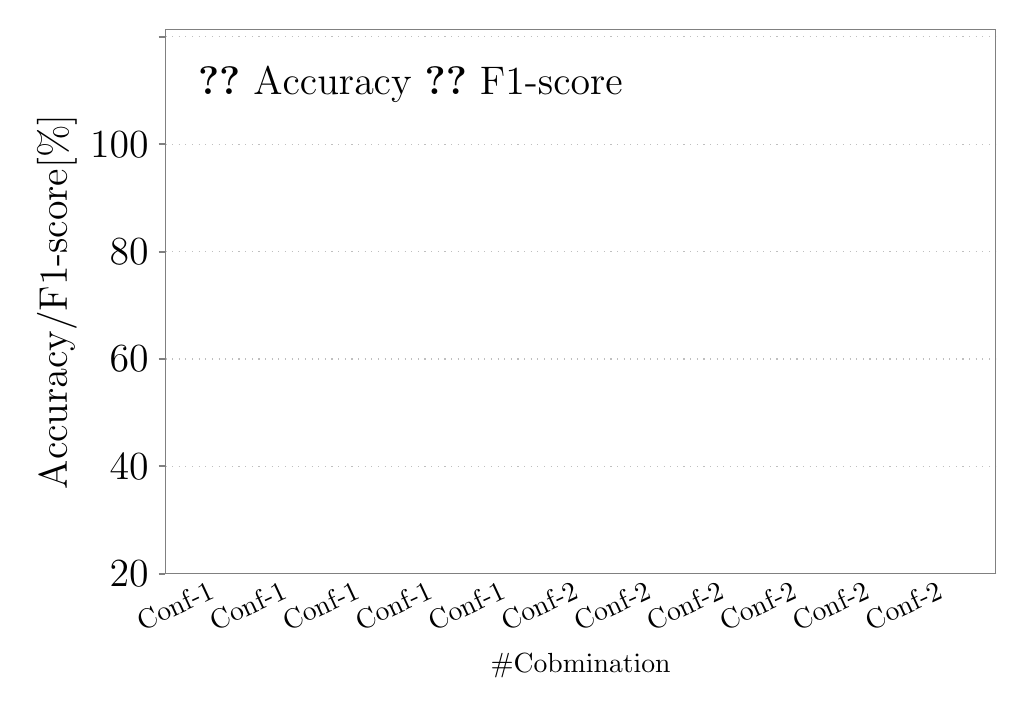
\begin{tikzpicture}[
  %ymode=log,  
  every axis/.style={
    major x tick style = {draw=none},
    %ybar stacked,
    %ymode=log,
    xtick style={draw=none},		
    every major tick/.append style={ thick,major tick length=2.5pt, gray},
    axis line style={gray},
    ybar,        
    ybar=0pt,
    ymin=0,
    ymax=1,
    log ticks with fixed point,
    y tick label style={/pgf/number format/1000 sep={}},
    x tick label style={/pgf/number format/1000 sep={}},
    scaled y ticks=false,
    enlarge y limits={0.013,upper},
    enlarge x limits=0.07,
    ylabel={Accuracy/F1-score[\%]},
    xlabel={$\#$Cobmination},
    ytick={0,0.2,0.4,0.6,0.8,1.0},
    yticklabels={0,20,40,60,80,100},
    ytick align=outside,
    xtick pos=left,
    ytick pos=left,
    yticklabel style = {font=\Large},
    ylabel style = {font=\Large, yshift=-2pt},
    xticklabel style = {font=\normalsize, xshift=-15pt, yshift=5pt, rotate=25},
    height=0.7\columnwidth,
    width=1\columnwidth,    
    bar width=5pt,	 
    ymajorgrids=true,
    grid style=dotted,   
    minor grid style={gray!50}, 
    xtick = data,
    symbolic x coords={Conf-1,Conf-2,Conf-3,Conf-4,Conf-5,Conf-6,Conf-7,Conf-8,Conf-9,Conf-10},
    legend image code/.code={\draw [#1] (0cm,-0.1cm) rectangle (0.2cm,0.3cm); },
  }	 ]
	
\begin{axis}%[hide axis]  
  \addplotCatDB{0}{gpt-4}{binary}{Abalone}{}{tug}{Accuracy};
\end{axis}


\node [draw=none,inner sep=0, font=\Large, anchor=west] (leg1) at (rel axis cs: 0.10,0.9) {\shortstack[l]{
			\ref{leg_pip_accuracy} Accuracy 
      \ref{leg_pip_f1_score} F1-score 			 			
	}};

\end{tikzpicture}


    %     \caption{Accuracy}
    % \end{figure}  
    
    
    % \tikzsetnextfilename{CatDB-Incremental-Binary_Albert}
    % \begin{figure}[h]
    %     \centering
    %     \newcommand{\addplotCatDB}[7]{
	   \addplot[xshift=#1,draw=black,line width=0.15pt, fill=tug, discard if singlecatdb={#2}{#3}{#4},postaction={#5}] 
	   table[ y=Accuracy, col sep=comma, x=prompt_representation_type] {results/Experiment_CatDB_Micro_Benchmark.dat};
	   \label{leg_pip_accuracy}     
     
     \addplot[xshift=0pt,draw=black,line width=0.15pt, fill=tugb, fill opacity=1, discard if singlecatdb={#2}{#3}{#4},postaction={#5}] 
	   table[ y=F1_score, col sep=comma, x=prompt_representation_type] {results/Experiment_CatDB_Micro_Benchmark.dat};
	   \label{leg_pip_f1_score}     
};

\pgfplotsset{
    discard if singlecatdb/.style n args={3}{
        x filter/.code={
            \edef\tempa{\thisrow{llm_model}}
            \edef\tempb{#1}
            \ifx\tempa\tempb
                    \edef\tempc{\thisrow{task_type}}
                    \edef\tempd{#2}
                    \ifx\tempc\tempd
                      \edef\tempe{\thisrow{dataset}}
                      \edef\tempf{#3}
                      \ifx\tempe\tempf                        	
                      \else
                      \def\pgfmathresult{inf}
                      \fi
                    \else
                    \def\pgfmathresult{inf}
                    \fi      
            \else
            \def\pgfmathresult{inf}
            \fi			
        }
    },
    discard if singleautoml/.style n args={2}{
      x filter/.code={
          \edef\tempa{\thisrow{framework}}
          \edef\tempb{#1}
          \ifx\tempa\tempb
                  \edef\tempc{\thisrow{type}}
                  \edef\tempd{#2}
                  \ifx\tempc\tempd   
                  \else                
                  \def\pgfmathresult{inf}
                  \fi      
          \else
          \def\pgfmathresult{inf}
          \fi			
      }
  }
};

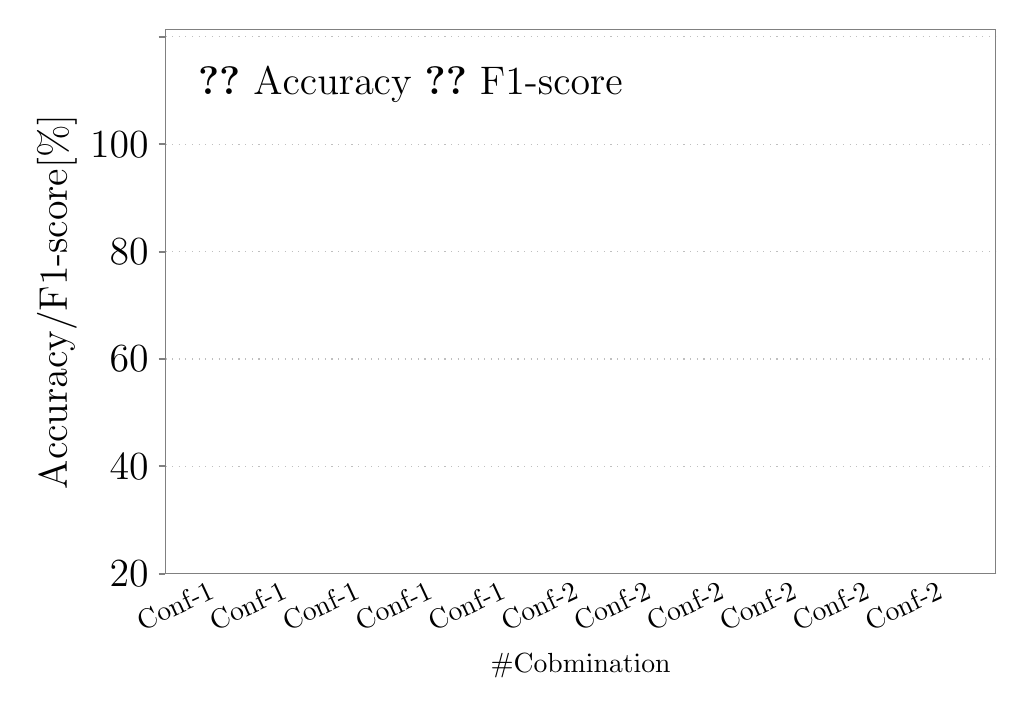
\begin{tikzpicture}[
  %ymode=log,  
  every axis/.style={
    major x tick style = {draw=none},
    %ybar stacked,
    %ymode=log,
    xtick style={draw=none},		
    every major tick/.append style={ thick,major tick length=2.5pt, gray},
    axis line style={gray},
    ybar,        
    ybar=0pt,
    ymin=0,
    ymax=1,
    log ticks with fixed point,
    y tick label style={/pgf/number format/1000 sep={}},
    x tick label style={/pgf/number format/1000 sep={}},
    scaled y ticks=false,
    enlarge y limits={0.013,upper},
    enlarge x limits=0.07,
    ylabel={Accuracy/F1-score[\%]},
    xlabel={$\#$Cobmination},
    ytick={0,0.2,0.4,0.6,0.8,1.0},
    yticklabels={0,20,40,60,80,100},
    ytick align=outside,
    xtick pos=left,
    ytick pos=left,
    yticklabel style = {font=\Large},
    ylabel style = {font=\Large, yshift=-2pt},
    xticklabel style = {font=\normalsize, xshift=-15pt, yshift=5pt, rotate=25},
    height=0.7\columnwidth,
    width=1\columnwidth,    
    bar width=5pt,	 
    ymajorgrids=true,
    grid style=dotted,   
    minor grid style={gray!50}, 
    xtick = data,
    symbolic x coords={Conf-1,Conf-2,Conf-3,Conf-4,Conf-5,Conf-6,Conf-7,Conf-8,Conf-9,Conf-10},
    legend image code/.code={\draw [#1] (0cm,-0.1cm) rectangle (0.2cm,0.3cm); },
  }	 ]
	
\begin{axis}%[hide axis]  
  \addplotCatDB{0}{gpt-4}{binary}{Albert}{}{tug}{Accuracy};
\end{axis}


\node [draw=none,inner sep=0, font=\Large, anchor=west] (leg1) at (rel axis cs: 0.10,0.9) {\shortstack[l]{
			\ref{leg_pip_accuracy} Accuracy 
      \ref{leg_pip_f1_score} F1-score 			 			
	}};

\end{tikzpicture}

    %     \caption{Accuracy}
    % \end{figure}  

    % \tikzsetnextfilename{CatDB-Incremental-Binary_Credit-g}
    % \begin{figure}[h]
    %     \centering
    %     \newcommand{\addplotCatDB}[7]{
	   \addplot[xshift=#1,draw=black,line width=0.15pt, fill=tug, discard if singlecatdb={#2}{#3}{#4},postaction={#5}] 
	   table[ y=Accuracy, col sep=comma, x=prompt_representation_type] {results/Experiment_CatDB_Micro_Benchmark.dat};
	   \label{leg_pip_accuracy}     
     
     \addplot[xshift=0pt,draw=black,line width=0.15pt, fill=tugb, fill opacity=1, discard if singlecatdb={#2}{#3}{#4},postaction={#5}] 
	   table[ y=F1_score, col sep=comma, x=prompt_representation_type] {results/Experiment_CatDB_Micro_Benchmark.dat};
	   \label{leg_pip_f1_score}     
};

\pgfplotsset{
    discard if singlecatdb/.style n args={3}{
        x filter/.code={
            \edef\tempa{\thisrow{llm_model}}
            \edef\tempb{#1}
            \ifx\tempa\tempb
                    \edef\tempc{\thisrow{task_type}}
                    \edef\tempd{#2}
                    \ifx\tempc\tempd
                      \edef\tempe{\thisrow{dataset}}
                      \edef\tempf{#3}
                      \ifx\tempe\tempf                        	
                      \else
                      \def\pgfmathresult{inf}
                      \fi
                    \else
                    \def\pgfmathresult{inf}
                    \fi      
            \else
            \def\pgfmathresult{inf}
            \fi			
        }
    },
    discard if singleautoml/.style n args={2}{
      x filter/.code={
          \edef\tempa{\thisrow{framework}}
          \edef\tempb{#1}
          \ifx\tempa\tempb
                  \edef\tempc{\thisrow{type}}
                  \edef\tempd{#2}
                  \ifx\tempc\tempd   
                  \else                
                  \def\pgfmathresult{inf}
                  \fi      
          \else
          \def\pgfmathresult{inf}
          \fi			
      }
  }
};

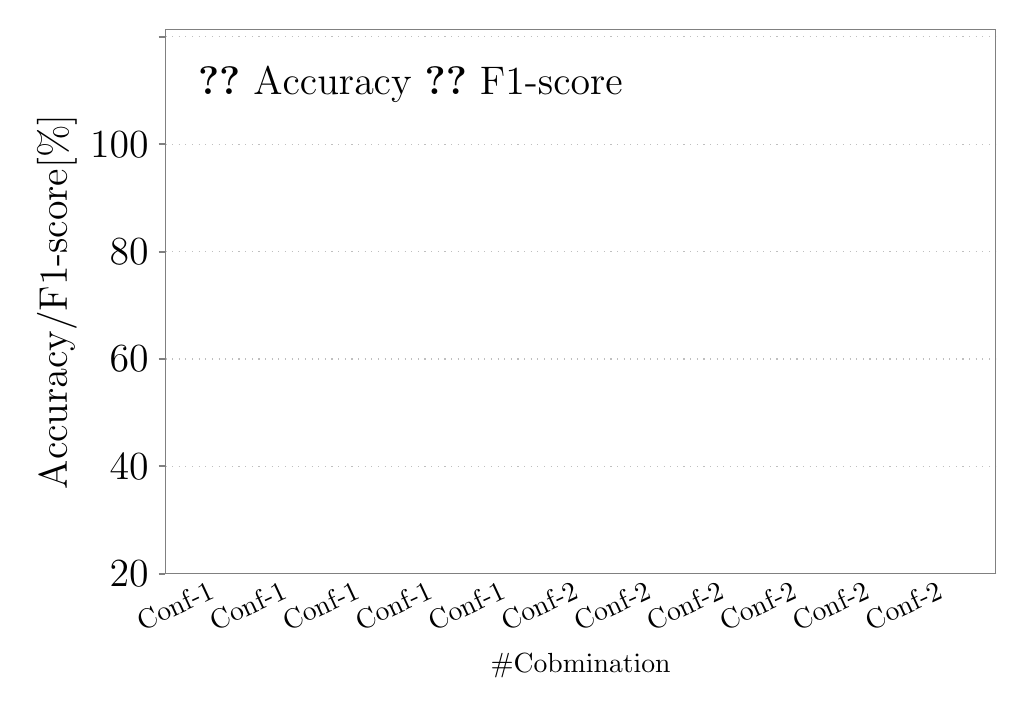
\begin{tikzpicture}[
  %ymode=log,  
  every axis/.style={
    major x tick style = {draw=none},
    %ybar stacked,
    %ymode=log,
    xtick style={draw=none},		
    every major tick/.append style={ thick,major tick length=2.5pt, gray},
    axis line style={gray},
    ybar,        
    ybar=0pt,
    ymin=0,
    ymax=1,
    log ticks with fixed point,
    y tick label style={/pgf/number format/1000 sep={}},
    x tick label style={/pgf/number format/1000 sep={}},
    scaled y ticks=false,
    enlarge y limits={0.013,upper},
    enlarge x limits=0.07,
    ylabel={Accuracy/F1-score[\%]},
    xlabel={$\#$Cobmination},
    ytick={0,0.2,0.4,0.6,0.8,1.0},
    yticklabels={0,20,40,60,80,100},
    ytick align=outside,
    xtick pos=left,
    ytick pos=left,
    yticklabel style = {font=\Large},
    ylabel style = {font=\Large, yshift=-2pt},
    xticklabel style = {font=\normalsize, xshift=-15pt, yshift=5pt, rotate=25},
    height=0.7\columnwidth,
    width=1\columnwidth,    
    bar width=5pt,	 
    ymajorgrids=true,
    grid style=dotted,   
    minor grid style={gray!50}, 
    xtick = data,
    symbolic x coords={Conf-1,Conf-2,Conf-3,Conf-4,Conf-5,Conf-6,Conf-7,Conf-8,Conf-9,Conf-10},
    legend image code/.code={\draw [#1] (0cm,-0.1cm) rectangle (0.2cm,0.3cm); },
  }	 ]
	
\begin{axis}%[hide axis]  
  \addplotCatDB{0}{gpt-4}{binary}{Credit-g}{}{tug}{Accuracy};
\end{axis}


\node [draw=none,inner sep=0, font=\Large, anchor=west] (leg1) at (rel axis cs: 0.10,0.9) {\shortstack[l]{
			\ref{leg_pip_accuracy} Accuracy 
      \ref{leg_pip_f1_score} F1-score 			 			
	}};

\end{tikzpicture}

    %     \caption{Accuracy}
    % \end{figure}  

    % \tikzsetnextfilename{CatDB-Incremental-Binary_Horsecolic}
    % \begin{figure}[h]
    %     \centering
    %     \newcommand{\addplotCatDB}[7]{
	   \addplot[xshift=#1,draw=black,line width=0.15pt, fill=tug, discard if singlecatdb={#2}{#3}{#4},postaction={#5}] 
	   table[ y=Accuracy, col sep=comma, x=prompt_representation_type] {results/Experiment_CatDB_Micro_Benchmark.dat};
	   \label{leg_pip_accuracy}     
     
     \addplot[xshift=0pt,draw=black,line width=0.15pt, fill=tugb, fill opacity=1, discard if singlecatdb={#2}{#3}{#4},postaction={#5}] 
	   table[ y=F1_score, col sep=comma, x=prompt_representation_type] {results/Experiment_CatDB_Micro_Benchmark.dat};
	   \label{leg_pip_f1_score}     
};

\pgfplotsset{
    discard if singlecatdb/.style n args={3}{
        x filter/.code={
            \edef\tempa{\thisrow{llm_model}}
            \edef\tempb{#1}
            \ifx\tempa\tempb
                    \edef\tempc{\thisrow{task_type}}
                    \edef\tempd{#2}
                    \ifx\tempc\tempd
                      \edef\tempe{\thisrow{dataset}}
                      \edef\tempf{#3}
                      \ifx\tempe\tempf                        	
                      \else
                      \def\pgfmathresult{inf}
                      \fi
                    \else
                    \def\pgfmathresult{inf}
                    \fi      
            \else
            \def\pgfmathresult{inf}
            \fi			
        }
    },
    discard if singleautoml/.style n args={2}{
      x filter/.code={
          \edef\tempa{\thisrow{framework}}
          \edef\tempb{#1}
          \ifx\tempa\tempb
                  \edef\tempc{\thisrow{type}}
                  \edef\tempd{#2}
                  \ifx\tempc\tempd   
                  \else                
                  \def\pgfmathresult{inf}
                  \fi      
          \else
          \def\pgfmathresult{inf}
          \fi			
      }
  }
};

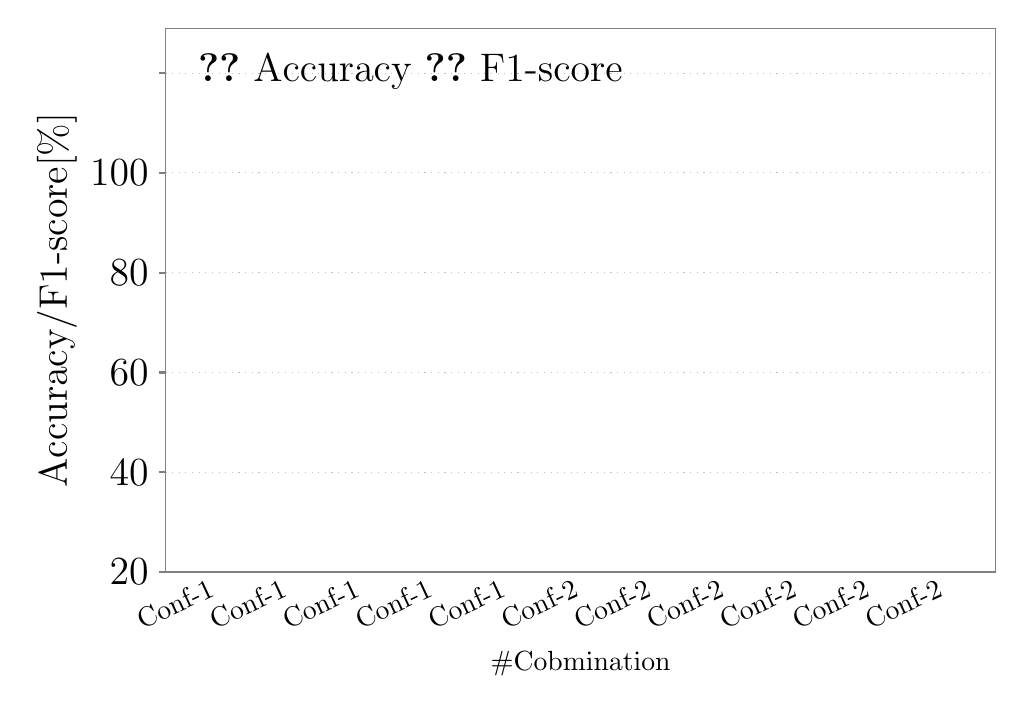
\begin{tikzpicture}[
  %ymode=log,  
  every axis/.style={
    major x tick style = {draw=none},
    %ybar stacked,
    %ymode=log,
    xtick style={draw=none},		
    every major tick/.append style={ thick,major tick length=2.5pt, gray},
    axis line style={gray},
    ybar,        
    ybar=0pt,
    ymin=0,
    ymax=1,
    log ticks with fixed point,
    y tick label style={/pgf/number format/1000 sep={}},
    x tick label style={/pgf/number format/1000 sep={}},
    scaled y ticks=false,
    enlarge y limits={0.09,upper},
    enlarge x limits=0.07,
    ylabel={Accuracy/F1-score[\%]},
    xlabel={$\#$Cobmination},
    ytick={0,0.2,0.4,0.6,0.8,1.0},
    yticklabels={0,20,40,60,80,100},
    ytick align=outside,
    xtick pos=left,
    ytick pos=left,
    yticklabel style = {font=\Large},
    ylabel style = {font=\Large, yshift=-2pt},
    xticklabel style = {font=\normalsize, xshift=-15pt, yshift=5pt, rotate=25},
    height=0.7\columnwidth,
    width=1\columnwidth,    
    bar width=5pt,	 
    ymajorgrids=true,
    grid style=dotted,   
    minor grid style={gray!50}, 
    xtick = data,
    symbolic x coords={Conf-1,Conf-2,Conf-3,Conf-4,Conf-5,Conf-6,Conf-7,Conf-8,Conf-9,Conf-10},
    legend image code/.code={\draw [#1] (0cm,-0.1cm) rectangle (0.2cm,0.3cm); },
  }	 ]
	
\begin{axis}%[hide axis]  
  \addplotCatDB{0}{gpt-4}{binary}{Horsecolic}{}{tug}{Accuracy};
\end{axis}


\node [draw=none,inner sep=0, font=\Large, anchor=west] (leg1) at (rel axis cs: 0.10,0.92) {\shortstack[l]{
			\ref{leg_pip_accuracy} Accuracy 
      \ref{leg_pip_f1_score} F1-score 			 			
	}};

\end{tikzpicture}

    %     \caption{Accuracy}
    % \end{figure}  

    % \tikzsetnextfilename{CatDB-Incremental-Binary_Sonar}
    % \begin{figure}[h]
    %     \centering
    %     \newcommand{\addplotCatDB}[7]{
	   \addplot[xshift=#1,draw=black,line width=0.15pt, fill=tug, discard if singlecatdb={#2}{#3}{#4},postaction={#5}] 
	   table[ y=Accuracy, col sep=comma, x=prompt_representation_type] {results/Experiment_CatDB_Micro_Benchmark.dat};
	   \label{leg_pip_accuracy}     
     
     \addplot[xshift=0pt,draw=black,line width=0.15pt, fill=tugb, fill opacity=1, discard if singlecatdb={#2}{#3}{#4},postaction={#5}] 
	   table[ y=F1_score, col sep=comma, x=prompt_representation_type] {results/Experiment_CatDB_Micro_Benchmark.dat};
	   \label{leg_pip_f1_score}     
};

\pgfplotsset{
    discard if singlecatdb/.style n args={3}{
        x filter/.code={
            \edef\tempa{\thisrow{llm_model}}
            \edef\tempb{#1}
            \ifx\tempa\tempb
                    \edef\tempc{\thisrow{task_type}}
                    \edef\tempd{#2}
                    \ifx\tempc\tempd
                      \edef\tempe{\thisrow{dataset}}
                      \edef\tempf{#3}
                      \ifx\tempe\tempf                        	
                      \else
                      \def\pgfmathresult{inf}
                      \fi
                    \else
                    \def\pgfmathresult{inf}
                    \fi      
            \else
            \def\pgfmathresult{inf}
            \fi			
        }
    },
    discard if singleautoml/.style n args={2}{
      x filter/.code={
          \edef\tempa{\thisrow{framework}}
          \edef\tempb{#1}
          \ifx\tempa\tempb
                  \edef\tempc{\thisrow{type}}
                  \edef\tempd{#2}
                  \ifx\tempc\tempd   
                  \else                
                  \def\pgfmathresult{inf}
                  \fi      
          \else
          \def\pgfmathresult{inf}
          \fi			
      }
  }
};

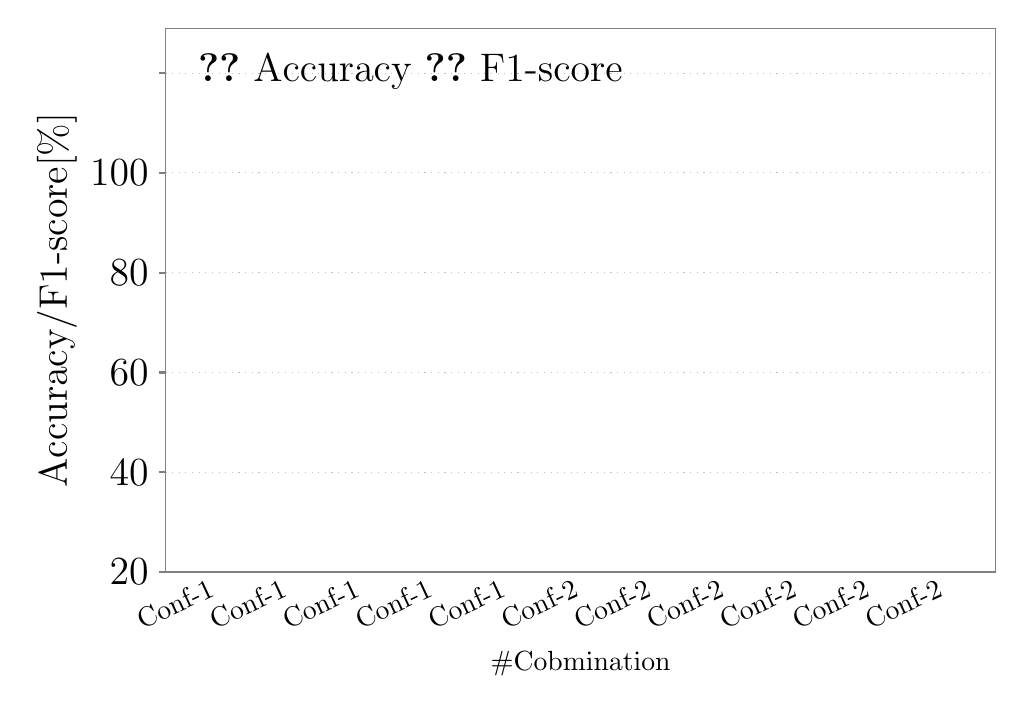
\begin{tikzpicture}[
  %ymode=log,  
  every axis/.style={
    major x tick style = {draw=none},
    %ybar stacked,
    %ymode=log,
    xtick style={draw=none},		
    every major tick/.append style={ thick,major tick length=2.5pt, gray},
    axis line style={gray},
    ybar,        
    ybar=0pt,
    ymin=0,
    ymax=1,
    log ticks with fixed point,
    y tick label style={/pgf/number format/1000 sep={}},
    x tick label style={/pgf/number format/1000 sep={}},
    scaled y ticks=false,
    enlarge y limits={0.09,upper},
    enlarge x limits=0.07,
    ylabel={Accuracy/F1-score[\%]},
    xlabel={$\#$Cobmination},
    ytick={0,0.2,0.4,0.6,0.8,1.0},
    yticklabels={0,20,40,60,80,100},
    ytick align=outside,
    xtick pos=left,
    ytick pos=left,
    yticklabel style = {font=\Large},
    ylabel style = {font=\Large, yshift=-2pt},
    xticklabel style = {font=\normalsize, xshift=-15pt, yshift=5pt, rotate=25},
    height=0.7\columnwidth,
    width=1\columnwidth,    
    bar width=5pt,	 
    ymajorgrids=true,
    grid style=dotted,   
    minor grid style={gray!50}, 
    xtick = data,
    symbolic x coords={Conf-1,Conf-2,Conf-3,Conf-4,Conf-5,Conf-6,Conf-7,Conf-8,Conf-9,Conf-10},
    legend image code/.code={\draw [#1] (0cm,-0.1cm) rectangle (0.2cm,0.3cm); },
  }	 ]
	
\begin{axis}%[hide axis]  
  \addplotCatDB{0}{gpt-4}{binary}{Sonar}{}{tug}{Accuracy};
\end{axis}


\node [draw=none,inner sep=0, font=\Large, anchor=west] (leg1) at (rel axis cs: 0.10,0.92) {\shortstack[l]{
			\ref{leg_pip_accuracy} Accuracy 
      \ref{leg_pip_f1_score} F1-score 			 			
	}};

\end{tikzpicture}



    %     \caption{Accuracy}
    % \end{figure}  

    \tikzsetnextfilename{CatDB-Incremental-Binary_Poker}
    \begin{figure}[h]
        \centering
        \newcommand{\addplotCatDB}[7]{
	   \addplot[xshift=#1,draw=black,line width=0.15pt, fill=tug, discard if singlecatdb={#2}{#3}{#4},postaction={#5}] 
	   table[ y=Accuracy, col sep=comma, x=prompt_representation_type] {results/Experiment_CatDB_Micro_Benchmark.dat};
	   \label{leg_pip_accuracy}     
     
     \addplot[xshift=0pt,draw=black,line width=0.15pt, fill=tugb, fill opacity=1, discard if singlecatdb={#2}{#3}{#4},postaction={#5}] 
	   table[ y=F1_score, col sep=comma, x=prompt_representation_type] {results/Experiment_CatDB_Micro_Benchmark.dat};
	   \label{leg_pip_f1_score}     
};

\pgfplotsset{
    discard if singlecatdb/.style n args={3}{
        x filter/.code={
            \edef\tempa{\thisrow{llm_model}}
            \edef\tempb{#1}
            \ifx\tempa\tempb
                    \edef\tempc{\thisrow{task_type}}
                    \edef\tempd{#2}
                    \ifx\tempc\tempd
                      \edef\tempe{\thisrow{dataset}}
                      \edef\tempf{#3}
                      \ifx\tempe\tempf                        	
                      \else
                      \def\pgfmathresult{inf}
                      \fi
                    \else
                    \def\pgfmathresult{inf}
                    \fi      
            \else
            \def\pgfmathresult{inf}
            \fi			
        }
    },
    discard if singleautoml/.style n args={2}{
      x filter/.code={
          \edef\tempa{\thisrow{framework}}
          \edef\tempb{#1}
          \ifx\tempa\tempb
                  \edef\tempc{\thisrow{type}}
                  \edef\tempd{#2}
                  \ifx\tempc\tempd   
                  \else                
                  \def\pgfmathresult{inf}
                  \fi      
          \else
          \def\pgfmathresult{inf}
          \fi			
      }
  }
};

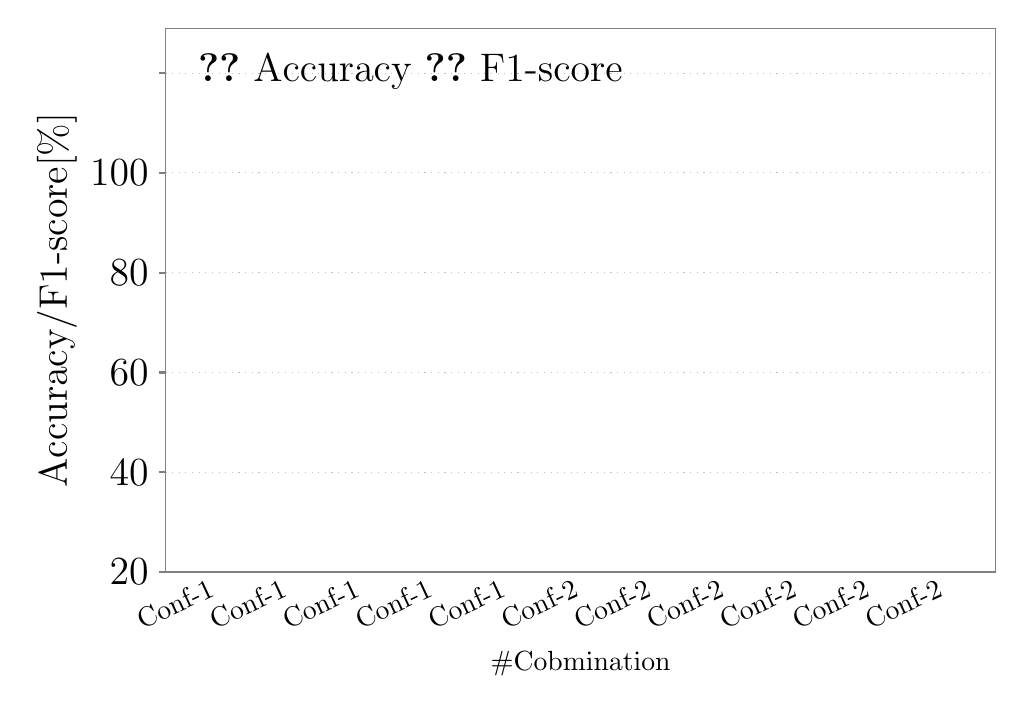
\begin{tikzpicture}[
  %ymode=log,  
  every axis/.style={
    major x tick style = {draw=none},
    %ybar stacked,
    %ymode=log,
    xtick style={draw=none},		
    every major tick/.append style={ thick,major tick length=2.5pt, gray},
    axis line style={gray},
    ybar,        
    ybar=0pt,
    ymin=0,
    ymax=1,
    log ticks with fixed point,
    y tick label style={/pgf/number format/1000 sep={}},
    x tick label style={/pgf/number format/1000 sep={}},
    scaled y ticks=false,
    enlarge y limits={0.09,upper},
    enlarge x limits=0.07,
    ylabel={Accuracy/F1-score[\%]},
    xlabel={$\#$Cobmination},
    ytick={0,0.2,0.4,0.6,0.8,1.0},
    yticklabels={0,20,40,60,80,100},
    ytick align=outside,
    xtick pos=left,
    ytick pos=left,
    yticklabel style = {font=\Large},
    ylabel style = {font=\Large, yshift=-2pt},
    xticklabel style = {font=\normalsize, xshift=-15pt, yshift=5pt, rotate=25},
    height=0.7\columnwidth,
    width=1\columnwidth,    
    bar width=5pt,	 
    ymajorgrids=true,
    grid style=dotted,   
    minor grid style={gray!50}, 
    xtick = data,
    symbolic x coords={Conf-1,Conf-2,Conf-3,Conf-4,Conf-5,Conf-6,Conf-7,Conf-8,Conf-9,Conf-10},
    legend image code/.code={\draw [#1] (0cm,-0.1cm) rectangle (0.2cm,0.3cm); },
  }	 ]
	
\begin{axis}%[hide axis]  
  \addplotCatDB{0}{gpt-4}{binary}{Poker}{}{tug}{Accuracy};
\end{axis}


\node [draw=none,inner sep=0, font=\Large, anchor=west] (leg1) at (rel axis cs: 0.10,0.92) {\shortstack[l]{
			\ref{leg_pip_accuracy} Accuracy 
      \ref{leg_pip_f1_score} F1-score 			 			
	}};

\end{tikzpicture}

        \caption{Accuracy}
    \end{figure}     
   

\end{document}
\endinput
